% Propósito: mostrar cómo la relación entre longitud de onda y barrera
% modifica la llegada a una zona sin línea de vista.
% Origen: comparación cualitativa para una geometría fija; no se asigna
% ninguna atenuación ni se representan datos experimentales.
% Accesibilidad: dos paneles comparan longitud de onda grande y pequeña;
% el rodeo del borde es más marcado en el primer caso.
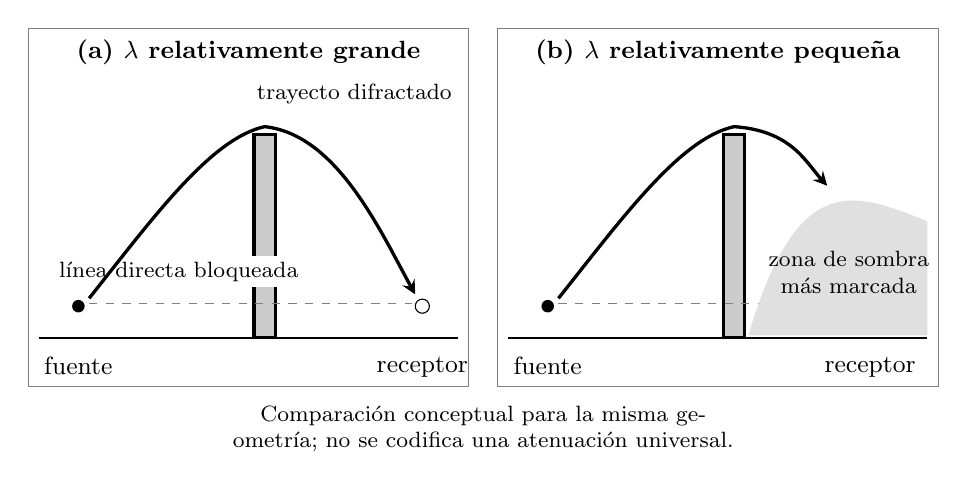
\begin{tikzpicture}[
    x=0.91cm,
    y=1cm,
    >=stealth,
    font=\small,
    camino/.style={very thick,->},
    directo/.style={gray,dashed}
]
    % Longitud de onda grande
    \draw[gray] (0,0) rectangle (6.15,4.55);
    \node[font=\small\bfseries] at (3.075,4.25)
        {(a) \(\lambda\) relativamente grande};
    \draw[thick] (0.15,0.62) -- (6.0,0.62);
    \draw[very thick,fill=black!20] (3.15,0.62) rectangle (3.45,3.20);
    \node[fill=black,circle,inner sep=1.6pt] (s1) at (0.70,1.02) {};
    \node[anchor=north] at (0.70,0.50) {fuente};
    \node[draw,circle,inner sep=1.8pt] (r1) at (5.50,1.02) {};
    \node[anchor=north] at (5.50,0.50) {receptor};
    \draw[directo] (0.85,1.05) -- (5.35,1.05);
    \node[fill=white,font=\footnotesize,inner sep=2pt]
        at (2.10,1.46) {línea directa bloqueada};
    \draw[camino] (0.85,1.12)
        .. controls (1.75,2.15) and (2.55,3.15) .. (3.30,3.30)
        .. controls (4.30,3.20) and (4.90,2.00) .. (5.40,1.17);
    \node[font=\footnotesize,fill=white,inner sep=2pt]
        at (4.55,3.72) {trayecto difractado};

    % Longitud de onda pequeña
    \draw[gray] (6.55,0) rectangle (12.70,4.55);
    \node[font=\small\bfseries] at (9.625,4.25)
        {(b) \(\lambda\) relativamente pequeña};
    \draw[thick] (6.70,0.62) -- (12.55,0.62);
    \draw[very thick,fill=black!20] (9.70,0.62) rectangle (10.00,3.20);
    \node[fill=black,circle,inner sep=1.6pt] (s2) at (7.25,1.02) {};
    \node[anchor=north] at (7.25,0.50) {fuente};
    \node[draw,circle,inner sep=1.8pt] (r2) at (11.75,1.02) {};
    \node[anchor=north] at (11.75,0.50) {receptor};
    \draw[directo] (7.40,1.05) -- (11.60,1.05);
    \draw[camino] (7.40,1.12)
        .. controls (8.30,2.15) and (9.10,3.15) .. (9.85,3.30)
        .. controls (10.65,3.25) and (10.85,2.85) .. (11.15,2.55);
    \path[fill=black!12] (10.05,0.65) -- (12.55,0.65) -- (12.55,2.10)
        .. controls (11.55,2.45) and (10.75,2.80) .. cycle;
    \node[align=center,font=\footnotesize] at (11.45,1.45)
        {zona de sombra\\más marcada};

    \node[font=\footnotesize,anchor=north,text width=11cm,align=center]
        at (6.35,-0.12)
        {Comparación conceptual para la misma geometría; no se codifica una atenuación universal.};
\end{tikzpicture}
